\section{Materials and Methods}
    
    \frame{\sectionpage}

    \begin{frame}{Trial Structure}
    
    \begin{columns}

    \begin{column}{0.7\textwidth}
        \begin{figure}\label{fig:trial_structure}
        \centering
        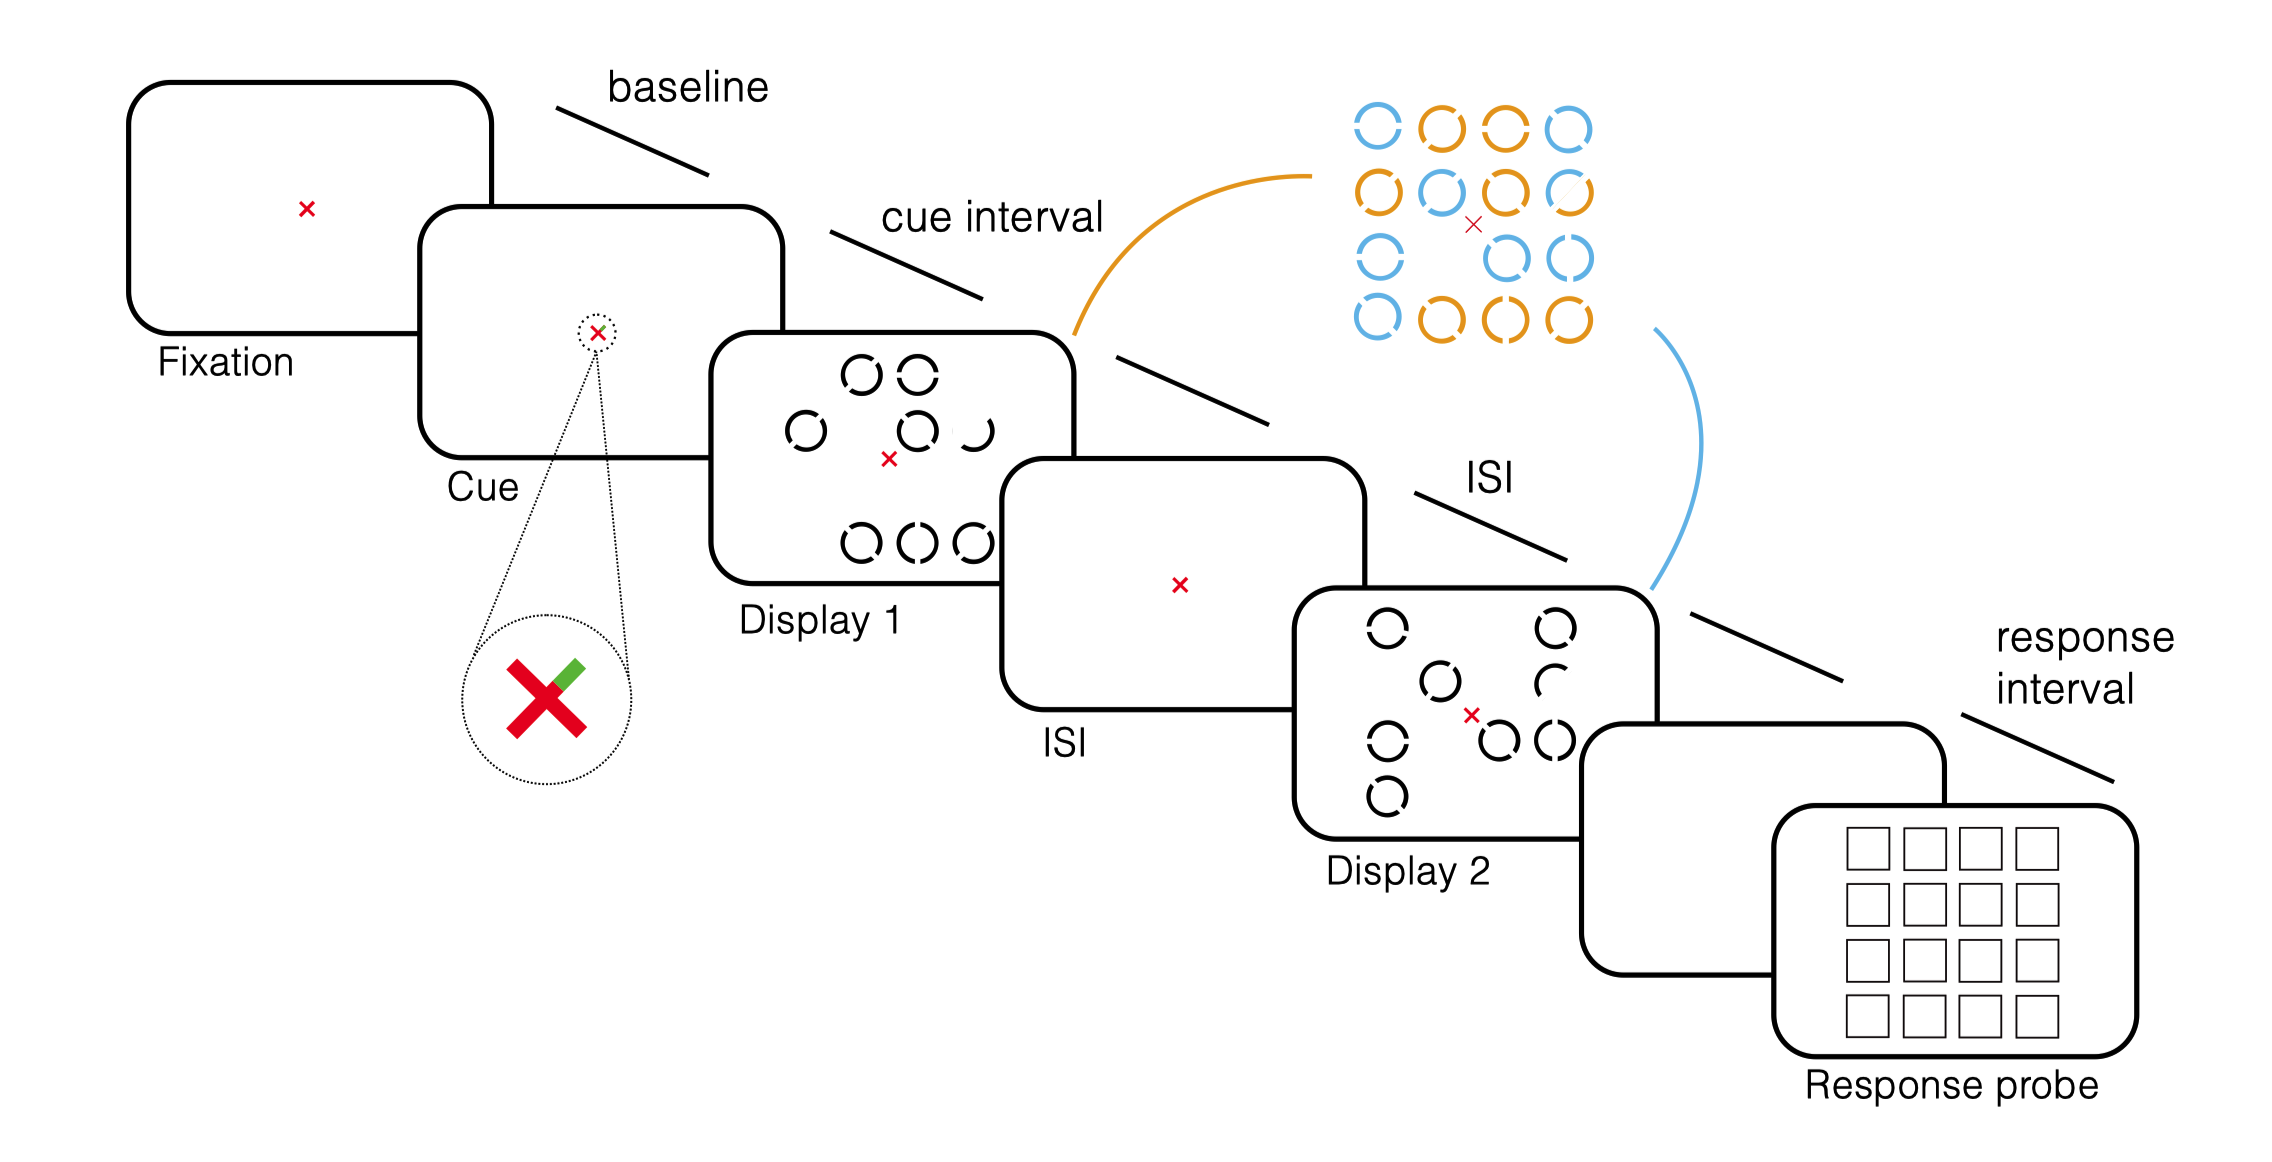
\includegraphics[height = 0.65 \textheight]{images/fig2_1.png}
        \caption{Trial Structure}
        \end{figure}
    \end{column}
    
    \begin{column}{0.25\textwidth}

    \only<2>{
        \small
        Timeline:
        \begin{itemize}
            \item pre-cue: 1000-1500ms
            \item cue interval: 850-1350ms (randomized)
            \item display: 16.67ms
            \item ISI: 48.3ms
            \item response delay: 400ms 
        \end{itemize}
        }
    
    \only<3>{
    \small
    visual cue: \textcolor{red}{\textbf{red}} cross
    \begin{itemize}
        \item 75\% (T): one of the arms turn \textcolor{green}{\textbf{green}}
        
        {\footnotesize (75\% valid)}
        \item 25\% (C): neutral cue
    \end{itemize}
    }

    \only<4>{
    \small
    2 displays: complementary, non-overlapping
    \begin{itemize}
        \item \underline{neutral cue}: the 2 displays \textcolor{lightlavender}{\textbf{complete}} each other
        \item \underline{empty}: one left \textcolor{lightlavender}{\textbf{empty}} in both
    \end{itemize}
    }

    \only<5>{
    \small
    task: moving a highlighted square
    \begin{itemize}
        \item \textcolor{lightlavender}{\textbf{\underline{segregation}}}: targeting the half circle
        \item \textcolor{lightlavender}{\textbf{\underline{integration}}}: targeting the empty spot
    \end{itemize}
    }
    
    \end{column}
    \end{columns}

    \end{frame}

\begin{frame}{Measures}

    \begin{columns}[T]

        \begin{column}{0.45\textwidth}
            \uncover<1->{\begin{block}{\small \centering \textbf{Eye tracking}}
            \uncover<2->{\footnotesize
            \begin{itemize}
                \item sampling rate: 1kHz
                \item rejection: 
                \begin{itemize}
                    \item[-] saccades: 7$\pm$7\% trials
                    \item[-] blinks: 3$\pm$4\% trials
                \end{itemize}
            \end{itemize}
            }
            \end{block}}
        \end{column}
        
        \begin{column}{0.45\textwidth}
            \uncover<1->{\begin{block}{\small \centering \textbf{MEG recording}}
            \uncover<3->{\footnotesize
            \begin{itemize}
                \item estimate instantaneous $\alpha-$frequency: 7- to 14-Hz frequency band
                \item rejection
                \begin{itemize}
                    \item[-] nonbiological noise: 10$\pm$1 channels 
                \end{itemize}
            \end{itemize}
            }
            \end{block}}
        \end{column}
        
        \end{columns}
    
\end{frame}


\begin{frame}{Analysis}

    \begin{columns}[T]

        \begin{column}{0.45\textwidth}
            \uncover<1->{\begin{block}{\small \centering \textbf{Source analysis}}
            \uncover<2->{\footnotesize
            \begin{itemize}
                \item combine head digitization data with \textcolor{lightlavender}{\underline{\textbf{anatomic MRI}}} data
                \item regions of interest:
                {
                    \begin{itemize}
                        \footnotesize
                    \item[-] parietal cortex
                    \item[-] occipital cortex
                \end{itemize}}
            \end{itemize}
            }
            \end{block}}
        \end{column}
        
        \begin{column}{0.45\textwidth}
            \uncover<1->{\begin{block}{\small \centering \textbf{Numerical analysis}}
            \uncover<3->{\footnotesize
            \begin{itemize}
                \item method: 2-way repeated ANOVA
                \item noise of raw estimates of $\alpha$ frequency: center on results following a \textcolor{lightlavender}{\textbf{\underline{neutral-cue}}}
                \begin{itemize}\footnotesize
                    \item[-] within each of the integration/segragation conditions separately
                \end{itemize}
            \end{itemize}
            }
            \end{block}}
        \end{column}
        
        \end{columns}
    
\end{frame}
    

    \begin{frame}{Other technical details}
        \begin{itemize}
            \item<+-> Participants: 29 (\textcolor{lightlavender}{\textbf{normal/corrected-to-normal}} vision; age 24$\pm$2.7 years; 11 male, 18 female)
            \item<+-> Stimuli: projected at 120Hz onto a translucent screen, at a viewing distance of \textcolor{lightlavender}{\textbf{1m}}
            \item<+-> Pre-MEG: 30 practice trials to achieve at least 25\% accuracy
            \item<+-> Number of trials: 10 blocks $\times$ 67 trials/block
            \item<+-> Base for numerical analysis: a shift in the \textcolor{lightlavender}{\textbf{neutral-cue}} baseline emerges equally in \textcolor{lightlavender}{\textbf{ipsilateral}} and \textcolor{lightlavender}{\textbf{contralateral}} signals
        \end{itemize}
        
    \end{frame}
